\documentclass[12pt,a4paper]{article}
\usepackage{tikz}
\usepackage{times}
\usepackage[left=3cm, right=2cm, top=3cm, bottom=3cm]{geometry}
\usetikzlibrary{circuits.plc.sfc,calc,positioning}
\usetikzlibrary{circuits.plc.ladder} 
\usepackage[utf8]{vietnam}
 \tikzset{
    coil NA/.style={coil={#1,symbol={$/$}}},
    every coil/.style={minimum size=2.4\tikzcircuitssizeunit,coil ladder curvature=0.5},
    every coil S/.style={minimum size=2.4\tikzcircuitssizeunit,coil ladder curvature=0.5},
    every coil R/.style={minimum size=2.4\tikzcircuitssizeunit,coil ladder curvature=0.5},
    every coil NA/.style={minimum size=2.4\tikzcircuitssizeunit,coil ladder curvature=0.5}
}
\usepackage{circuitikz}
\usepackage{indentfirst}
\setlength{\parindent}{0cm}
\begin{document}

{\Large
\textbf{\LARGE Bài tập nhóm \#2}


\begin{tabbing}{}
    \setlength{\parindent}{1cm}
    Tên nhóm A \= Điều khiển góc phương vị của chảo vệ tinh \kill
    \textbf{Tên nhóm} \> l'Automatisation
\end{tabbing}
}


\section{Mạch điều khiển}

\begin{figure}[h!]
    \centering
    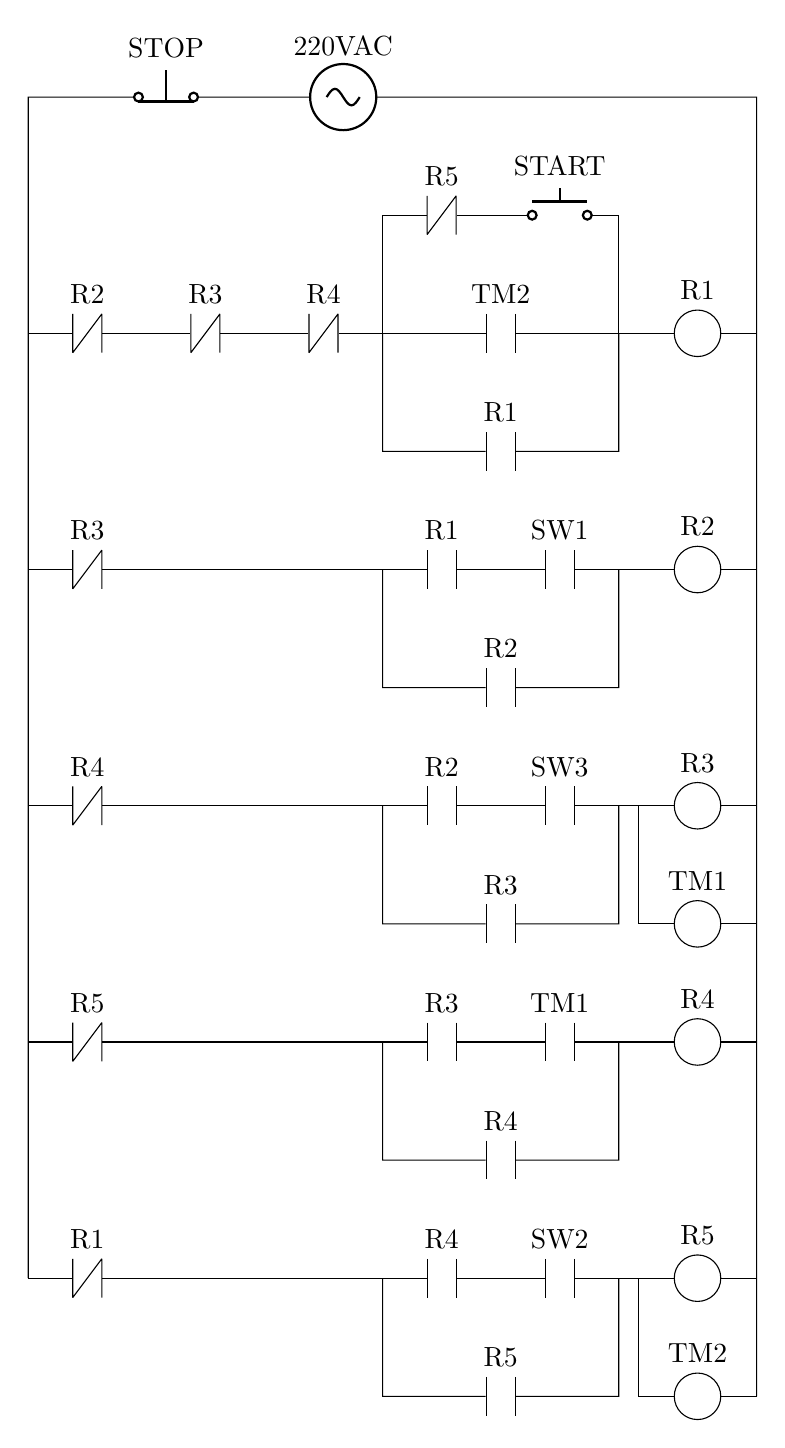
\begin{tikzpicture}[circuit plc ladder,x=1cm,y=1cm]
        \draw (1.5,0) to[contact NC={info=R2}] ++ (1.5,0)
            to[contact NC={info=R3}] ++ (1.5,0)
            to[contact NC={info=R4}] ++ (1.5,0) coordinate(R1)
            to[contact NO={info=TM2}] ++ (3,0) -- ++(0.25,0)
            to[coil={info=R1}] ++ (1.5,0);
        \draw (R1) -- ++(0,1.5) 
            to[contact NC={info=R5}] ++ (1.5,0)
            to[nopb,l=START] ++ (1.5,0) -- ++(0,-1.5);
        \draw (R1) -- ++(0,-1.5) to[contact NO={info=R1}] ++ (3,0) -- ++(0,1.5);
        

        \draw (1.5,-3) to [contact NC={info=R3}] ++(1.5,0) -- ++(3,0) coordinate (R2)
            to[contact NO={info=R1}] ++ (1.5,0)
            to[contact NO={info=SW1}] ++ (1.5,0) -- ++(0.25,0)
            to[coil={info=R2}] ++ (1.5,0);
        \draw (R2) -- ++(0,-1.5) to[contact NO={info=R2}] ++ (3,0) -- ++(0,1.5);

        \draw (1.5,-6) to [contact NC={info=R4}] ++(1.5,0) -- ++(3,0) coordinate (R3)
            to[contact NO={info=R2}] ++ (1.5,0)
            to[contact NO={info=SW3}] ++ (1.5,0) -- ++(0.25,0) coordinate (R3c)
            to[coil={info=R3}] ++ (1.5,0);
        \draw (R3) -- ++(0,-1.5) to[contact NO={info=R3}] ++ (3,0) -- ++(0,1.5);
        \draw (R3c) -- ++(0,-1.5) to[coil={info=TM1}] ++ (1.5,0);

        \draw (1.5,-9) to [contact NC={info=R5}] ++(1.5,0) -- ++(3,0) coordinate (R4)
            to[contact NO={info=R3}] ++ (1.5,0)
            to[contact NO={info=TM1}] ++ (1.5,0) -- ++(0.25,0)
            to[coil={info=R4}] ++ (1.5,0);
        \draw (R4) -- ++(0,-1.5) to[contact NO={info=R4}] ++ (3,0) -- ++(0,1.5);

        \draw (1.5,-12) to [contact NC={info=R1}] ++(1.5,0) -- ++(3,0) coordinate (R5)
            to[contact NO={info=R4}] ++ (1.5,0)
            to[contact NO={info=SW2}] ++ (1.5,0) -- ++(0.25,0) coordinate (R5c)
            to[coil={info=R5}] ++ (1.5,0);
        \draw (R5) -- ++(0,-1.5) to[contact NO={info=R5}] ++ (3,0) -- ++(0,1.5);
        \draw (R5c) -- ++(0,-1.5) to[coil={info=TM2}] ++ (1.5,0);


        \draw (1.5,-12) |- ++(1,15) to[ncpb,l=STOP] ++ (1.5,0) --++(1.5,0) coordinate (V) -- ++ (1,0) -| (10.75,-13.5);

        \node[vsourcesinshape, rotate=90, scale=1,fill=white] at (V) {};
        \node[above=4mm] at (V) {220VAC};
    \end{tikzpicture}
    \caption{Sơ đồ mạch điều khiển}
    \label{fig:my_label}
\end{figure}
\end{document}